%=========================================================================================================
% References: https://tex.stackexchange.com/questions/196957/how-can-i-draw-this-cycloid-diagram-with-tikz
%=========================================================================================================

\documentclass[tikz,border=15pt]{standalone}
\usepackage{tikz}
\begin{document}
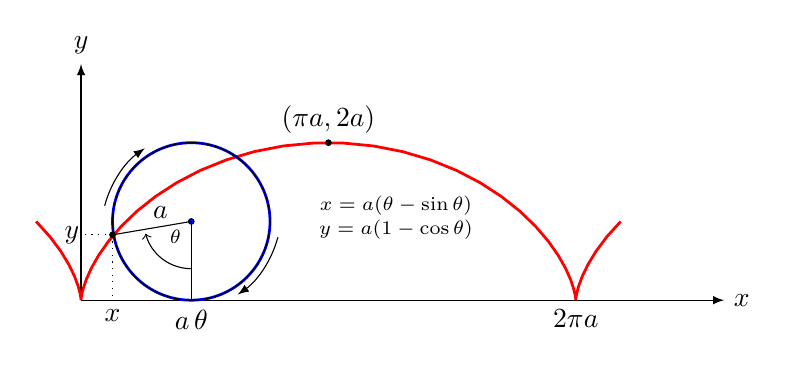
\begin{tikzpicture}
\coordinate (O) at (0,0);
\coordinate (A) at (0,3);
\def\r{1} % radius
\def\c{1.4} % center
\coordinate (C) at (\c, \r);

\draw[-latex] (O) -- (A) node[anchor=south] {$y$};
\draw[-latex] (O) -- (2.6*pi,0) node[anchor=west] {$x$};
\draw[red,domain=-0.5*pi:2.5*pi,samples=50, line width=1] 
   plot ({\x - sin(\x r)},{1 - cos(\x r)});
\draw[blue, line width=1] (C) circle (\r);
\draw[] (C) circle (\r);

% coordinate x 
\def\x{0.4} % coordinate x
\def\y{0.83} % coordinate y
\def\xa{0.3} % coordinate x for arc left
\def\ya{1.2} % coordinate y for arc left
\coordinate (X) at (\x, 0 );
\coordinate (Y) at (0, \y );
\coordinate (XY) at (\x, \y );

\node[anchor=north] at (X) {$x$} ;

% draw center of circle
\draw[fill=blue] (C) circle (1pt);

% draw radius of the circle
\draw[] (C) -- node[anchor=south] {\; $a$} (XY);

% bottom of circle, radius to the bottom
\coordinate (B) at (\c, 0);
\draw[] (C) -- (B) node[anchor=north] {$a \, \theta$};

% projections of point XY
\draw[dotted] (XY) -- (X);
\draw[dotted] (XY) -- (Y) node[anchor=east, xshift=1mm] {$\quad y$};

% arc theta
% start arc
\coordinate (S) at (\c, 0.4);
\draw[->] (S) arc (-90:-165:0.6);
\node[xshift=-2mm, yshift=-2mm] at (C) {\scriptsize $\theta$};

% arc above
\coordinate (AA) at (\xa, \ya);
\draw[-latex, rotate=25] (AA) arc (-220:-260:1.3);

% arc below
\def\xb{2.5} % coordinate x for arc bottom
\def\yb{0.8} % coordinate y for arc bottom
\coordinate (AB) at (\xb, \yb);
\draw[-latex, rotate=-10] (AB) arc (-5:-45:1.3);

% XY dot
\draw[fill=black] (XY) circle (1pt);

% top label
\coordinate (T) at (pi, 2);
\node[anchor=south] at (T)  {$(\pi a, 2 a )$} ;
\draw[fill=black] (T) circle (1pt);

% equations
\coordinate (E) at ( 4,1.2);
\coordinate (F) at ( 4,0.9);
\node[] at (E) {\scriptsize $x=a(\theta - \sin \theta)$};
\node[] at (F) {\scriptsize $y=a(1 - \cos \theta)$};

% label 2pi a
\coordinate (TPA) at (2*pi, 0);
\node[anchor=north] at (TPA) {$2 \pi a$};
\end{tikzpicture}
\end{document}
